\documentclass[11pt]{article}
\usepackage[T1]{fontenc}
\usepackage{lmodern,microtype}
\usepackage[margin=1in]{geometry}
\usepackage{amsmath,amssymb,amsthm,booktabs,enumitem,needspace}
\usepackage{tikz,listings}
\usepackage[hidelinks,pdftitle={Leaf deletion can move the unique mode of a tree domination polynomial by two},pdfauthor={Dev D. Goyal}]{hyperref}
\newtheorem{theorem}{Theorem}
\newtheorem{lemma}[theorem]{Lemma}
\newtheorem{proposition}[theorem]{Proposition}
\newcommand{\D}{D}
\newcommand{\coeff}[2]{[x^{#1}]#2}
\lstset{language=Python,basicstyle=\ttfamily\scriptsize,columns=fullflexible,keepspaces=true,showstringspaces=false,breaklines=true,frame=single,aboveskip=8pt,belowskip=8pt}
\title{Leaf deletion can move the unique mode\\of a tree domination polynomial by two}
\author{Dev D. Goyal}
\date{}
\begin{document}
\maketitle
\paragraph{Autonomous AI research disclosure.}
This work is fully autonomous agentic research. Automated systems produced the research, proofs, formalization, and manuscript preparation. Dev D. Goyal is responsible for publication. No expert validation or peer review is claimed.

\begin{abstract}
Deleting one leaf of a tree need not move a mode of its domination polynomial by at most one, even when both coefficient sequences are unimodal. An explicit tree on $7284$ vertices has a unique mode at $3978$, while deleting a specified leaf produces a tree on $7283$ vertices with a unique mode at $3976$. The proof counts actual dominating subsets by conditioning on the central vertex, then checks a finite set of exact integer coefficient inequalities. A differential recurrence gives a short, reproducible arithmetic certificate. The graph semantics, polynomial identities, unimodality, unique modes, and actual induced leaf deletion are also formalized in Lean. The result concerns local mode stability; both witness polynomials are unimodal.
\end{abstract}

\section{The question and the witness}
A subset $A$ of the vertices of a finite simple graph $G$ is \emph{dominating} if every vertex belongs to $A$ or has a neighbor in $A$. The ordinary domination polynomial is
\[
 \D(G,x)=\sum_{\substack{A\subseteq V(G)\\A\text{ dominating}}}x^{|A|}
        =\sum_{j\ge0}d_j(G)x^j.
\]
Thus $d_j(G)$ counts dominating subsets of cardinality $j$. All coefficient sequences below include the zero coefficients beyond the degree. A sequence $(c_j)_{j\ge0}$ is \emph{unimodal at $m$} if $c_j\le c_{j+1}$ for $j<m$ and $c_{j+1}\le c_j$ for $j\ge m$. A \emph{mode} is any index of a global maximum. A unique mode is strictly larger than every coefficient at a different index.

The leaf-deletion question asks whether two unimodal domination polynomials of a tree and its leaf-deleted tree must have a pair of modes at distance at most one. The motivating question is attributed to Question~8.1 of Burcroff and O'Brien~\cite{burcroff}, and a related proximity conjecture to Zhang~\cite{zhang}. Those primary texts, question numbers, and current-version correspondence have not been verified here. The construction below refutes the explicitly stated proximity assertion. It resolves an external question only if its definitions and quantifiers agree with this assertion. Uniqueness makes the result independent of any convention for selecting a mode on a plateau. No priority claim or minimality claim is made.

For integers $n\ge0$ and $k\ge1$, construct $R_{n,k}$ with a central vertex $r$. For each $1\le i\le n$, introduce distinct vertices $u_i,v_i,w_{i,1},\ldots,w_{i,k}$. Add exactly the edges
\begin{equation}\label{eq:edges}
 \{r,u_i\},\qquad \{u_i,v_i\},\qquad
 \{v_i,w_{i,j}\}\quad(1\le i\le n,\ 1\le j\le k).
\end{equation}
Let $T_{n,k}$ be obtained by adding one new vertex $z$ and the edge $\{r,z\}$. Figure~\ref{fig:branch} displays one branch. All branches are disjoint away from $r$.

\begin{figure}[ht]
\centering
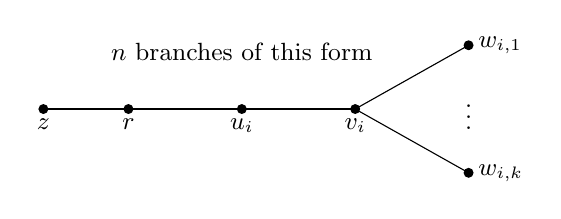
\begin{tikzpicture}[scale=0.9,every node/.style={font=\small}]
\draw (0,0)--(1.6,0)--(3.2,0);
\draw (0,0)--(-1.2,0);
\draw (3.2,0)--(4.8,0.9) (3.2,0)--(4.8,-0.9);
\foreach \x/\y/\name/\pos in {0/0/r/below,1.6/0/u_i/below,3.2/0/v_i/below,-1.2/0/z/below,4.8/0.9/{w_{i,1}}/right,4.8/-0.9/{w_{i,k}}/right}
 {\fill (\x,\y) circle (2pt);\node[\pos] at (\x,\y) {$\name$};}
\node at (4.8,0) {$\vdots$};
\node[above,align=center] at (1.6,0.55) {$n$ branches of this form};
\end{tikzpicture}
\caption{One branch of $T_{n,k}$ and its additional root leaf $z$. Deleting $z$ leaves $R_{n,k}$. The vertex $r$ is shared by the $n$ branches.}\label{fig:branch}
\end{figure}

\begin{theorem}\label{thm:main}
Let $T=T_{662,9}$, let $z$ be its additional root leaf, and let $R=T-z=R_{662,9}$. Then $T$ is a tree on $7284$ vertices, $z$ has degree one, and $R$ is a tree on $7283$ vertices. Both $\D(T,x)$ and $\D(R,x)$ are unimodal. Their unique modes are respectively $3978$ and $3976$. Consequently, no mode of one polynomial lies within distance one of a mode of the other.
\end{theorem}

Every vertex has a path to $r$. Every nonroot vertex has exactly one parent at a smaller depth, and the edges in~\eqref{eq:edges}, together with $rz$ when present, are exactly these parent edges. There is one edge per nonroot vertex, so the connected graphs are trees. Their orders are $1+n(k+2)$ and $2+n(k+2)$. The new vertex has the sole neighbor $r$, and its induced deletion is precisely $R_{n,k}$. It remains to establish the polynomial claims.

\section{Counting the dominating subsets}
The enumeration works for every $n\ge0$ and $k\ge1$. Introduce
\begin{equation}\label{eq:SU}
 S_k=(1+x)\bigl((1+x)^k+x^{k-1}\bigr),\qquad
 U_k=(1+x)^{k+1}+x^k.
\end{equation}
Each selected vertex contributes a factor $x$, and each optional vertex contributes $1+x$. A branch consists of $u_i,v_i$ and its $k$ tips, excluding $r$.

\begin{proposition}\label{prop:formula}
For the ordinary domination polynomials of the graphs above,
\begin{align}
 \D(R_{n,k},x)&=x^n\bigl(xS_k^n+U_k^n-(1+x)^{kn}\bigr),\label{eq:R}\\
 \D(T_{n,k},x)&=x^{n+1}\bigl((1+x)S_k^n+U_k^n\bigr).\label{eq:T}
\end{align}
\end{proposition}
\begin{proof}
First suppose $r$ is selected. Then $u_i$ is dominated already. If $v_i$ is selected, $u_i$ and all $k$ tips are optional, contributing $x(1+x)^{k+1}$. If $v_i$ is absent, all its tips must be selected, while $u_i$ remains optional, contributing $x^k(1+x)$. The hypothesis $k\ge1$ ensures that these tips also dominate $v_i$. The total branch contribution is therefore $xS_k$.

Suppose instead that $r$ is absent, and require all branch vertices to be dominated. If $v_i$ is selected, the contribution is again $x(1+x)^{k+1}$. If $v_i$ is absent, every tip and $u_i$ must be selected: each tip has no other neighbor, and $u_i$ has neither $r$ nor $v_i$ available to dominate it. This gives $x^{k+1}$. The branch contribution is $xU_k$.

For $R_{n,k}$, in the root-absent case the root fails to be dominated exactly when every $u_i$ is absent. In such a branch $v_i$ must be selected, with all tips optional, contributing $x(1+x)^k$. Independence of the disjoint branches now gives
\[
 \D(R_{n,k},x)=x(xS_k)^n+(xU_k)^n-
                    \bigl(x(1+x)^k\bigr)^n,
\]
which is~\eqref{eq:R}. The subtraction removes exactly the configurations that fail to dominate $r$, once each. This also covers $n=0$: the formula reduces to $x$, the polynomial of the one-vertex tree.

For $T_{n,k}$, when $r$ is selected the new leaf $z$ is optional, adding a factor $1+x$. When $r$ is absent, $z$ must be selected and then dominates $r$. Thus no root-domination exclusion is needed, and
\[
 \D(T_{n,k},x)=x(1+x)(xS_k)^n+x(xU_k)^n,
\]
which is~\eqref{eq:T}. These cases partition the actual vertex subsets. Their weights are $x$ to the cardinality of each subset, so the identities concern the ordinary domination polynomials.
\end{proof}

\section{The exact coefficient certificate}
Set $n=662$ and $k=9$, and abbreviate
\begin{align*}
 S&=(1+x)^{10}+x^8+x^9,& U&=(1+x)^{10}+x^9,\\
 F&=S^{662},&G&=U^{662},&H&=(1+x)^{5958},\\
 P&=xF+G-H,&Q&=(1+x)F+G.
\end{align*}
Proposition~\ref{prop:formula} gives
\begin{equation}\label{eq:shifts}
 \D(R,x)=x^{662}P,\qquad \D(T,x)=x^{663}Q.
\end{equation}
The coefficient vectors of $S$ and $U$, in ascending degree order, are
\begin{align*}
 s&=(1,10,45,120,210,252,210,120,46,11,1),\\
 u&=(1,10,45,120,210,252,210,120,45,11,1).
\end{align*}
Both $P$ and $Q$ have degree $6621$ and leading coefficient one. Write $f_j,g_j,h_j$ for the coefficients of $F,G,H$, setting them to zero for every index outside their supports, including negative indices. Then
\begin{equation}\label{eq:pqcoeff}
 p_j=f_{j-1}+g_j-h_j,\qquad
 q_j=f_{j-1}+f_j+g_j.
\end{equation}

The only large numerical step is a complete finite check of the adjacent inequalities in Table~\ref{tab:certificate}. All arithmetic uses integers. The next lemma explains exactly how to generate the coefficients, so the check does not require the printed expansion of three large powers.

\begin{lemma}[Differential recurrence]\label{lem:recurrence}
Let $A(x)=\sum_{i=0}^d a_i x^i\in\mathbb Z[x]$ with $a_0=1$, and let $N\ge1$. The coefficients $b_j=[x^j]A^N$ are uniquely determined by $b_0=1$ and
\begin{equation}\label{eq:recurrence}
 j b_j=\sum_{i=1}^{\min(d,j)}\bigl((N+1)i-j\bigr)a_i b_{j-i}
 \qquad(j\ge1).
\end{equation}
Only the values $0\le j\le dN$ are needed; all later coefficients vanish.
\end{lemma}
\begin{proof}
For $B=A^N$, differentiation gives $AB'=NA'B$. Equating coefficients of $x^{j-1}$ yields
\[
 \sum_{i=0}^{\min(d,j)}(j-i)a_i b_{j-i}
 =N\sum_{i=1}^{\min(d,j)}i a_i b_{j-i}.
\]
Isolating the $i=0$ term gives~\eqref{eq:recurrence}. Each right side uses only earlier coefficients, and multiplication by the nonzero integer $j$ is injective. Hence induction determines the coefficients uniquely. Existence follows from $A^N$, so every division in the recurrence is exact. The degree bound follows from polynomial multiplication.
\end{proof}

\begin{lemma}[Finite integer comparisons]\label{lem:finite}
The coefficients in~\eqref{eq:pqcoeff} are nonnegative and satisfy every comparison in Table~\ref{tab:certificate}. In particular, the indicated peak coefficients are positive.
\end{lemma}
\begin{proof}[Exact finite verification]
Apply~\eqref{eq:recurrence} to $(s,662)$, $(u,662)$ and $((1,1),5958)$, then form~\eqref{eq:pqcoeff} for $0\le j\le6621$. The complete program in Appendix~\ref{app:code} carries out these operations and tests every comparison. It uses only integer addition, multiplication, order, and division with remainder. Every remainder is checked to be zero. The program completed with all checks passing. Its loops cover all coefficients through degree $6621$ and the final comparison against the zero coefficient at degree $6622$; all later comparisons are $0\le0$. Thus the check is exhaustive over the infinite zero-extended sequences. A separate Lean certificate checks the polynomial identities and these inequalities by kernel reduction, as described in Section~\ref{sec:formal}.
\end{proof}

\begin{table}[ht]
\centering
\begin{tabular}{@{}lll@{}}
\toprule
Check & $P$ & $Q$\\\midrule
Increasing & $p_j\le p_{j+1}$, $0\le j<3314$ & $q_j\le q_{j+1}$, $0\le j<3315$\\
Decreasing & $p_{j+1}\le p_j$, $3314\le j$ & $q_{j+1}\le q_j$, $3315\le j$\\
Strict summit & $p_{3313}<p_{3314}>p_{3315}$ & $q_{3314}<q_{3315}>q_{3316}$\\
Positive summit & $0<p_{3314}$ & $0<q_{3315}$\\\bottomrule
\end{tabular}
\caption{The complete coefficient-shape certificate. Each decreasing range includes every natural-number index at or above its lower bound.}\label{tab:certificate}
\end{table}

\begin{proof}[Completion of the proof of Theorem~\ref{thm:main}]
Lemma~\ref{lem:finite} proves that $P$ is unimodal at $3314$. For $j<3314$, monotonicity gives $p_j\le p_{3313}<p_{3314}$. For $j>3314$, it gives $p_j\le p_{3315}<p_{3314}$. Hence $3314$ is the unique mode of $P$. The same argument gives the unique mode $3315$ of $Q$.

Multiplication by $x^a$ inserts $a$ initial zero coefficients. Since all coefficients are nonnegative, this preserves unimodality and translates its peak index by $a$. Since the peak is positive, none of the inserted zeros can be another mode. Equation~\eqref{eq:shifts} therefore gives the unique modes $662+3314=3976$ and $663+3315=3978$. Their difference is two. The tree and leaf claims were established after Theorem~\ref{thm:main}, completing all assertions.
\end{proof}

There is a useful indexing check. Although $\D(R,x)$ has a factor $x^{662}$, its coefficient at degree $662$ vanishes: $P(0)=0$ and $p_1=663>0$. Also $Q(0)=2$. Both ordinary domination polynomials therefore have exactly $663$ initial zero coefficients, at indices $0,\ldots,662$. The two shifts in~\eqref{eq:shifts} must still be kept distinct.

\section{Formal verification and scope}\label{sec:formal}
The formalization defines the domination polynomial as a sum over actual finite vertex subsets, with exponent equal to subset cardinality. Its coefficient theorem identifies each coefficient with the number of dominating subsets of that size. A bijection between subset choices and root/branch configurations proves the enumeration formulas. An explicit graph isomorphism identifies $R_{662,9}$ with the induced deletion of $z$ from $T_{662,9}$.

The numerical certificate stores the three ascending coefficient lists. It checks, for each proposed list $B$ and base $A$, the polynomial identity $AB'=NA'B$ and $B(0)=1$. To justify this method independently of a generator, suppose $B_1,B_2$ satisfy the same identity and constant term. Their difference $E$ satisfies $AE'=NA'E$ and $E(0)=0$. If all coefficients of $E$ below degree $j$ vanish, comparison at degree $j-1$ gives $j[x^j]E=0$, because $A(0)=1$. Induction gives $E=0$. Thus the checked lists are the actual powers. List operations are proved to implement polynomial addition, multiplication, differentiation and coefficient access. The shape checker then proves all adjacent inequalities, including the trailing zero, and the strict neighboring comparisons prove uniqueness.

The project uses Lean 4.19.0 and mathlib revision
\begin{center}\texttt{\small c44e0c8ee63ca166450922a373c7409c5d26b00b}.\end{center}
On 28 October 2026 a fresh build of the 18 scientific proof/data modules succeeded. A separate \texttt{-{}-trust=0} audit checked ten named endpoints. The reports use only \texttt{propext}, \texttt{Classical.choice}, and \texttt{Quot.sound}; the two complete coefficient-trend reports have no axiom dependencies. The numerical certificates use \texttt{decide +kernel}. The original scientific sources and toolchain pin were unchanged. The replay used a derived dependency lock at the exact mathlib revision specified by the original configuration, which did not contain a lock file. A declaration map and reproduction instructions accompany the manuscript.

The assembled theorem \texttt{LeafMode.Result.counterexample} includes the actual tree, its degree-one vertex, both unimodality statements, both unique modes, and exclusion of every pair of modes at distance at most one. The existential endpoint is \texttt{LeafMode.Result.question\_8\_1}. Its name refers to the package-defined statement and does not authenticate an external question number. Formal verification establishes these mathematical claims. It does not establish historical priority or the current status of the cited questions.

The witness shows why leaf-by-leaf induction cannot assume a mode shift of at most one under unimodality. It neither proves nor refutes unimodality of domination polynomials for all trees. No smallest witness, unbounded mode jump, or log-concavity theorem is asserted. Root-state enumeration is established counting machinery; no novelty of that method is claimed. Source comparisons and historical priority remain provisional.

\bibliographystyle{plain}
\bibliography{references}

\clearpage
\appendix
\section{Complete reproducible integer check}\label{app:code}
The following standard-library Python program is also supplied as \texttt{check\_coefficients.py}. Run it with ordinary \texttt{python3}. It rejects optimization mode, including optimization requested through the environment, so that its assertions cannot be silently disabled. A successful run prints \texttt{PASS} and the two graph modes. No coefficient data file or floating-point computation is used. The final two total-count identities are additional consistency checks at $x=1$.
\lstinputlisting{check_coefficients.py}
\end{document}
